\chapter{Results} \label{sec:results}
In this chapter we present the results of open-circuit simulations of the digital transformer.
An open circuit of a transformer is of particular interest, as it is generally used to determine core losses. 
We run the simulations for both the linear- as well as the non-linear model. 
All simulations are run with 
\begin{itemize}
    \item $I_s = 777.72$ A,
    \item $I_p = 0$ A,
    \item $N_s = 266$,
    \item $N_p = 6$,
    \item $f = 50$ Hz.
\end{itemize}
These are the parameters used in \cite{vanDijk2022}.

\section{Linear behaviour}
Taking $\mu_{r, core} = 1000 \frac{\text{H}}{\text{m}}$  and $\mu_{r, air} = 10 \frac{\text{H}}{\text{m}}$, \cref{fig:linear_model} shows the magnetic flux through all three core legs for three periods of the source signal. This can be viewed as the superposition of three contributions, one for each core leg
\begin{align*}
    B_{\text{left leg}} &= B_0\left(\sin(\omega t - \phi) - \sin(\omega t)\right), \\
    B_{\text{middle leg}} &= B_0\left(\sin(\omega t) - \sin(\omega t - \phi) - \sin(\omega t + \phi)\right), \\
    B_{\text{right leg}} &= B_0\left(\sin(\omega t + \phi) - \sin(\omega t)\right),
\end{align*}
where $B_0$ is the amplitude of the magnetic flux and $\phi$ is the phase shift of the three-phase source signal.
Note that this is only true for the linear model. The above equations are derived by realising that any
coil induces a magnetic flux in the core leg it is wrapped around and an opposing flux in its neighbouring legs. Plotting above expressions gives \cref{fig:linear_model_theory}. Comparing this to \cref{fig:linear_model}, it is clear that the linear model behaves as expected.
\begin{figure}
    \centering
    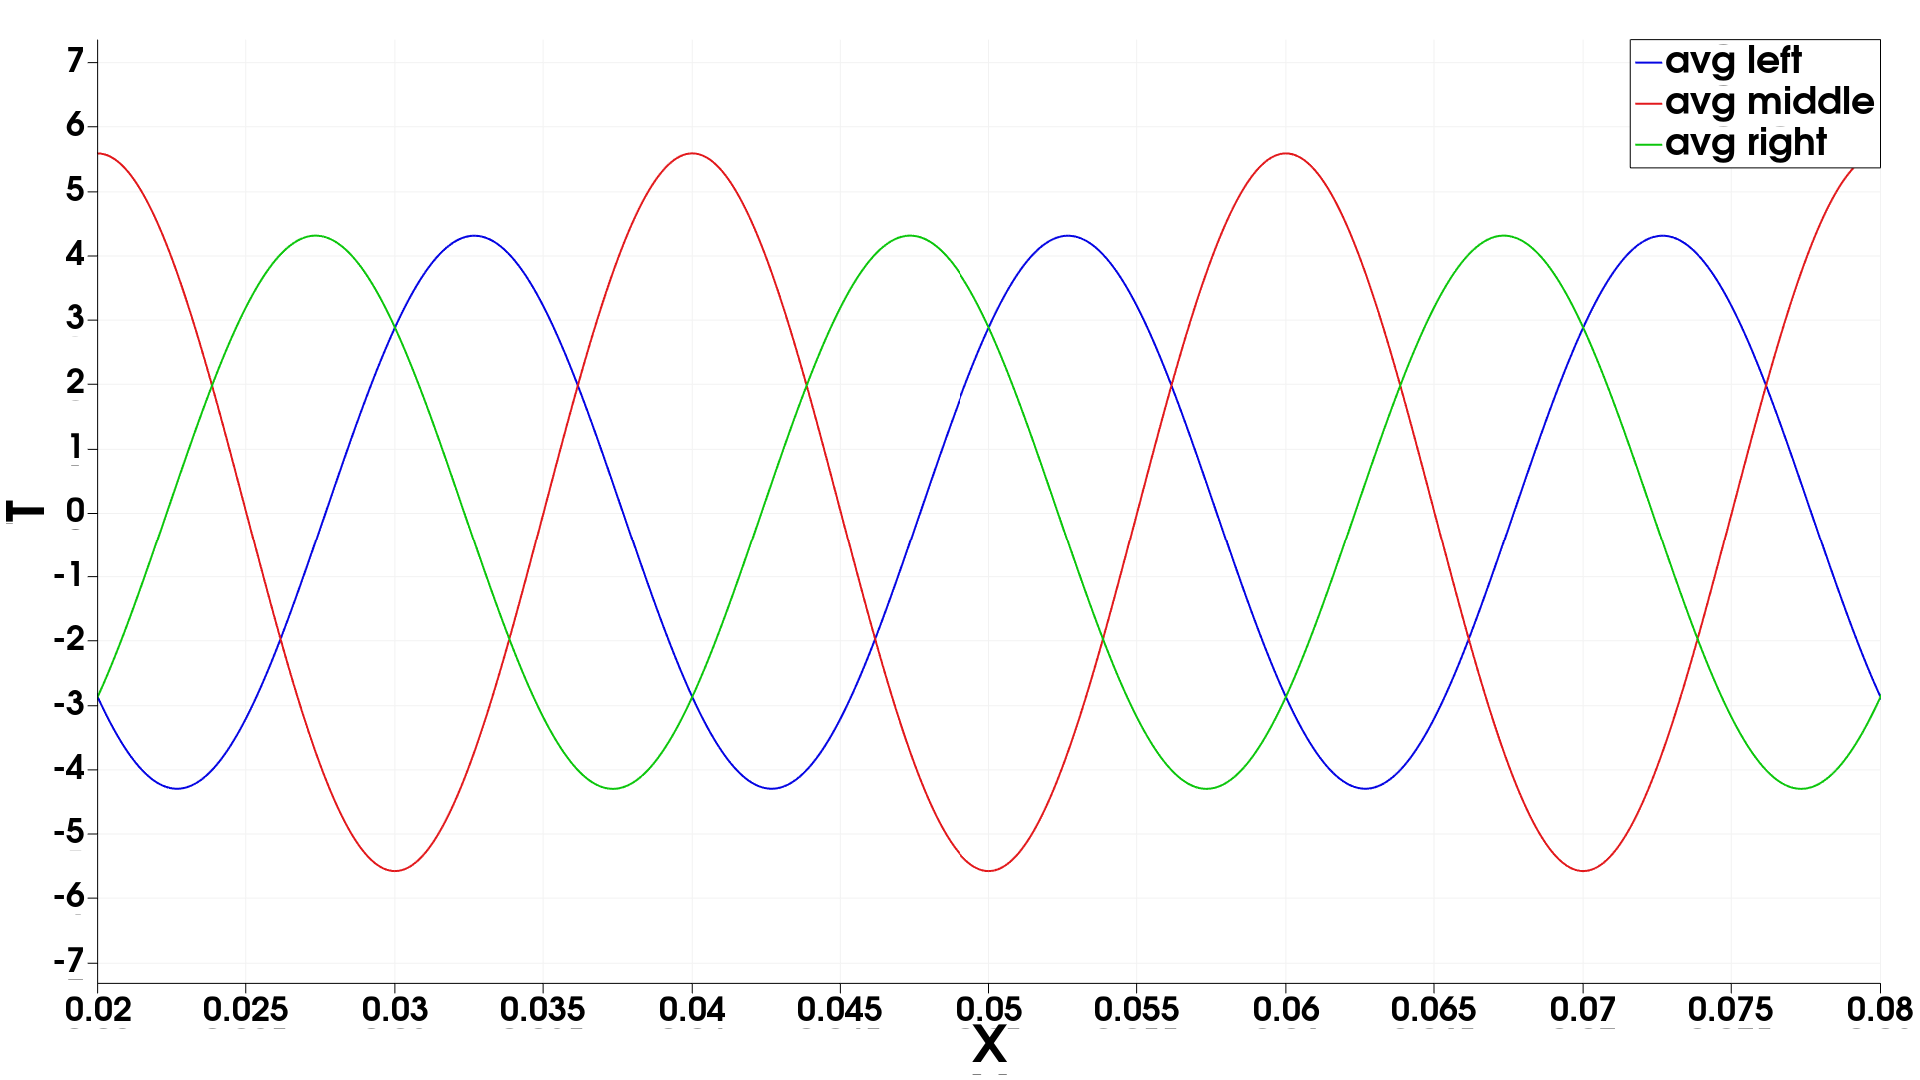
\includegraphics[width=0.7\textwidth]{img/B_phase_plot_linear_mu.png}
    \caption{Magnetic flux against time in all three core legs for the linear model.}
    \label{fig:linear_model}
\end{figure}
\begin{figure}
    \centering
    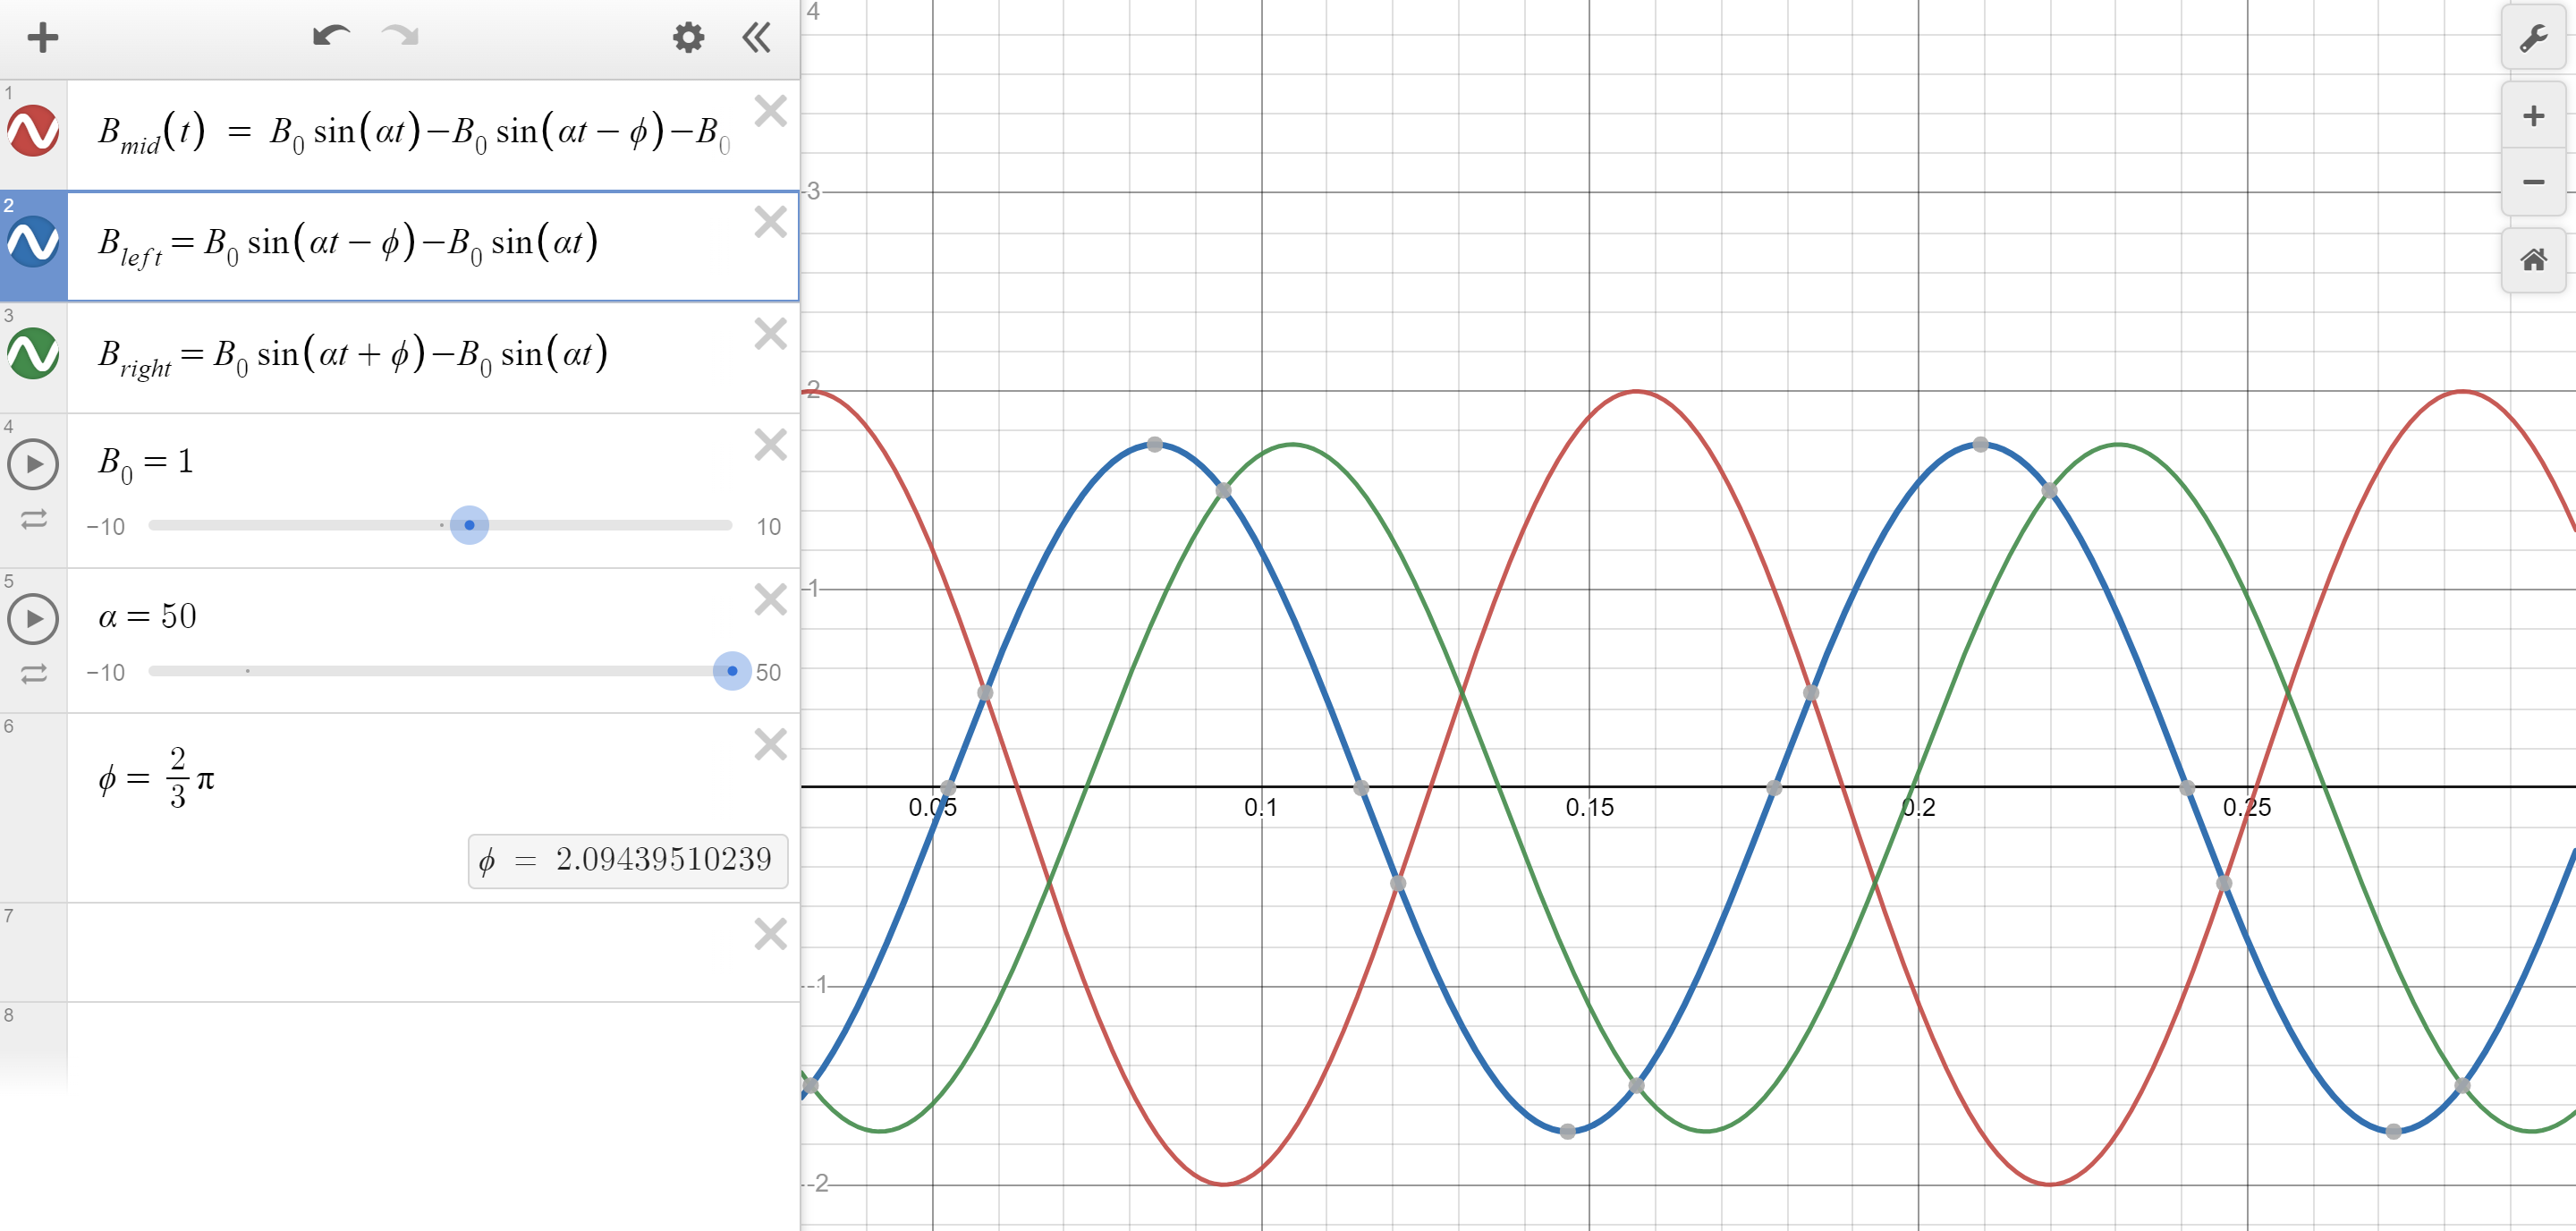
\includegraphics[width=0.7\textwidth]{img/Screenshot_68.png}
    \caption{Predicted magnetic flux against time in all three core legs for the linear model.}
    \label{fig:linear_model_theory}
\end{figure}
\begin{figure}
    \centering
    \includegraphics[width=0.7\textwidth]{phaseplot_b_nonlinear.eps}
    \caption{Phase plot of $B$ for the non-linear model.}
    \label{fig:nonlinear_phaseplot}
\end{figure}

\section{Non-linear behaviour}
We now take 
\begin{equation*}
\mu_{\text{core, r}}(||\textbf{B}||) = \left(\alpha + (1 - \alpha) \frac{||\textbf{B}||^{2\beta}}{||\textbf{B}||^{2\beta} + \gamma}\right)^{-1},
\end{equation*}
$\alpha = 2.12 \times 10^{-4}$, $\beta = 7.358$ and $\gamma = 1.18 \times 10^{-4}$.
which has a saturation point at $||\textbf{B}|| \approx 2$ T.
\cref{fig:nonlinear_phaseplot} shows the phase plot of $B$ for the non-linear model, which is quite different from the linear case.

Firstly, the magnetic flux rises much more sharply than in the linear case. This is expected, as the permeability of the core is higher than in the linear case because the core is unsaturated.

Secondly, the maximum magnetic flux is much lower than in the linear case, $\approx 2$T vs. $\approx 6$. This behaviour is also expected, as the saturation point of the core is reached, which means that the permeability of the core is much lower than in the linear case. This influences the magnetic flux, and is correctly captured by the non-linear model. This is visible in the plot by the quick flattening of the magnetic flux at e.g. 2 Tesla for the middle leg.

\vspace{10pt}

\noindent The full solution for the magnetic flux in all three core legs is shown in Figure \ref{fig:nonlinear_bnorm}. If we compare this with \cref{fig:steady_state}, we can interpret the differences between the models. One of the implications of the lower permeability, is that the flux can not penetrate that area of the core. In \cref{fig:steady_state} it can be seen that the flux rises to 12 Tesla near the inside corners; this is unrealistic. In the non-linear model, this is not the case. However, other parts of the iron core are still permeable, and therefore the flux can still penetrate there. This leads to nearly full saturation of the core at the cross-sections. This is much more realistic behaviour. 


\begin{figure}
    \centering
    \includegraphics[width=0.8\textwidth]{bnorm_t0.004.eps}
    \caption{$||B||$ at $t = 0.004$ s for the non-linear model.}
    \label{fig:nonlinear_bnorm}
\end{figure}


\begin{figure}
    \centering
    \includegraphics[width=0.7\textwidth]{img/b_field_steady_state2.png}
    \caption{$||B||$ at $t = 0.004$ s, for the linear model.}
    \label{fig:steady_state}
\end{figure}


This hypothesis can be confirmed by looking at a plot of the permeability, given in \cref{fig:nonlinear_permeability}. Thge permeability is very at the points where the flux is high, and low where the flux is low. This is exactly what we expect from the non-linear model.

\begin{figure}
    \centering
    \includegraphics[width=0.8\textwidth]{permeability_t0.004.eps}
    \caption{Permeability of the core at $t = 0.004$ s, for the non-linear model.}
    \label{fig:nonlinear_permeability}
\end{figure}


As a last test, we can look at the permeability as a function of the magnetic flux, given in \cref{fig:nonlinear_permeability_bnorm}. This is a plot of the permeability as a function of $||B||$. We see that the permeability is very high for low values of $||B||$, and then drops off quickly, as expected.

\begin{figure}
    \centering
    \includegraphics[width=0.8\textwidth]{permeability_nonlinear.eps}
    \caption{Permeability as a function of $||B||$.}
    \label{fig:nonlinear_permeability_bnorm}
\end{figure}





